\chapter{Introductions to QuickCheck}
\label{APP:QUICKCHECK}
\lstset{style=erlang}
\label{SEC:QuickCheckIntro}

\section{The General Idea}
The general idea with QuickCheck, is here explained using an example.
Lets say that one has a \emph{sort} function that takes a list $Xs$ of any
sortable items and returns the sorted version $Ys$ of $Xs$. To verify the
correctness of this function it is possible to look at certain properties
that must hold for a correctly implemented sort function. For instance:

\noindent The arity of $Y$ must be the same.
\begin{equation}
        |Xs| = |Ys|
\end{equation}

\noindent The elements of $Ys$ must actually be sorted.
\begin{equation}
    y_{i-1} \leq y_i, \forall y_i \in Ys, i \neq 0
\end{equation}

\noindent For all permutations $Pe(Xs)$ holds:
\begin{equation}
sort(Zs) = Ys, \forall Zs \in Pe(Xs)
\end{equation}

\noindent The sets $Xs$ and $Ys$ contains the same elements.
\begin{equation}
        x \in Xs \leftrightarrow x \in Ys
\end{equation}
Instead of specifying own test cases QuickCheck makes it possible to write such
properties, automatically generates test cases and checks that the properties
specified actually holds.

\section{Testing C-code}
QuickCheck is a testing tool for the programming language Erlang, but it is
possible to efficiently test C-code, using QuickCheck, by performing API-calls
against the C-code within Erlang.  Lets say that there is a \emph{Queue}
implementation in C that has a function for creating a new queue as well
as functions for inserting and retrieving elements from a queue structure.

\begin{lstlisting}[style=c]
typedef struct
{
   int size;
   int head;
   int tail;
   int* buffer;
} Queue;

Queue* new(int size) { ... }
int put(Queue* q, int element) { ... }
int get(Queue* q) { ... }
\end{lstlisting}
This program has a number of properties that should hold. For
instance:
\begin{itemize}
\item When creating a new queue, the C function should return an
address to the memory where it have allocated space.
\item The function \lstinline!put! should insert the element into the queue
and return the element.
\item It should be possible to dequeue an element in the order it was
inserted with the function \lstinline!get!.
\end{itemize}
Such properties can be used when using QuickCheck.
%Instead of specifying own test cases QuickCheck makes it possible to
%write such properties, automatically generates test cases and checks
%that the properties specified actually holds.

When testing C code with QuickCheck one uses state based
testing. Which means that a model state $S$ is passed around and
checked against API calls according to figure \ref{FIG:API_CALLS}.

\begin{figure}[!h]
  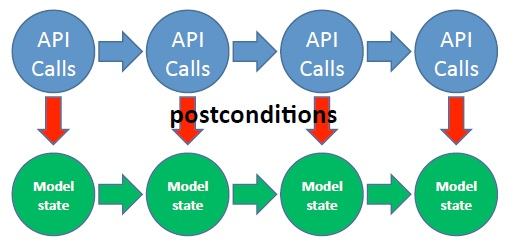
\includegraphics{pictures/api_calls.jpg}
  \caption{Shows state based testing against API and model state}
  \label{FIG:API_CALLS}
\end{figure}
First a model of the queue must be implemented in Erlang code.
It is also needed to implement a representation of the current state of the queue.

\begin{lstlisting}
-record(state, {ptr, queue}).

new_next(_S, Pointer, _) ->
   #state{ptr=Pointer, queue=[]}.
put_next(S, _, [_, X]) ->
   S#state{queue = S#state.queue++[X]}.
get_next(S, _, _) ->
   S#state{queue = tl(S#state.queue)}.
\end{lstlisting}

The \lstinline!record! will contain information needed to successfully
test the states of the program. It has two variables;
\emph{ptr} which is the pointer to the queue and
\emph{queue} which is a list defining all inserted elements in the queue.

QuickCheck must also be told how to call the C-functions.
\begin{lstlisting}
new(Size) ->
  q:new(Size).
put(Ptr, Val) ->
  q:put(Ptr, Val).
get(Ptr) ->
  q:get(Ptr).
\end{lstlisting}

Now the postconditions, program properties that must hold, are defined.
\begin{lstlisting}
new_post(_S, _Arguments, ReturnValue) ->
  case ReturnValue of
    {ptr, "Queue", _} -> true;
    _                 -> false
  end.
put_post(_S, [_, InsertedValue], ReturnValue) ->
  ReturnValue == InsertedValue.
get_post(S, _Arguments, ReturnValue) ->
  ReturnValue == hd(S#state.elements).
\end{lstlisting}

To be able to test these properties QuickCheck needs to know how to generate
arguments for every functions.
\begin{lstlisting}
new_args(_S) ->
   [nat()].
put_args(S) ->
   [S#state.ptr, int()].
get_args(S) ->
   [S#state.ptr].
\end{lstlisting}
The functions \lstinline!nat()! and \lstinline!int()! are generators
defined by QuickCheck to generate arbitrary natural numbers and integers.

To test the functions \emph{put}, \emph{get} and \emph{new} defined in the C-code a QuickCheck
property is written in the following way.  \lstset{style=erlang}
\begin{lstlisting}
prop() ->
  ?FORALL(Cmds, commands(),
          begin
            ... = run_commands(Cmds)
          end).
\end{lstlisting}

The function \emph{commands()} is a generator that looks
for functions defining the API-calls, such as \emph{new}, \emph{put} and
\emph{get}, in the Erlang module. The \emph{commands()} function then combines
every function $api_i$ defining an API-call with a function $arg_i$ which
generates the arguments to $api_i$.

After the property has been implemented, it can be tested by:

\begin{lstlisting}
eqc:quickcheck(prop()).
\end{lstlisting}

It is possible define how many tests QuickCheck should execute and also if the
states of the model should be shown:
\begin{lstlisting}
eqc:quickcheck(eqc:numtests(N, eqc_statem:show_states(prop()))).
\end{lstlisting}

\section{QuickCheck Modules}
QuickCheck consist of several Erlang modules.
%%eqc
\subsection{eqc}
The module \emph{eqc} is the main QuickCheck module. This module defines a lot
of macros that can be used when writing properties and also basic functions
like \emph{quickcheck}.

\subsection{eqc\_gen} The module is used for generation of test cases. The module
contains various functions and macros for this purpose. There are some
predefined generators, for instance for integers and characters etcetera, but it
is quite easy to construct a generator for almost any data type. Just to get the
idea follows code for a string generator.
\begin{lstlisting}
    ?LET(Pat, nat(), vector(Pat, char()))
\end{lstlisting}
The macro \emph{?LET} binds a generated value from the second argument, to \emph{Pat} which can be
used in the third argument. The above code binds a natural number, from the
generator \emph{nat()}, to \emph{Pat} and creates a vector with length
\emph{Pat} of characters.

A generator can also be weighted, or in other words certain values can be more
likely to be generated than others.

\begin{lstlisting}
?LET(Pat, nat(), vector(Pat,
                        frequency([{1, choose(0,127)},
                                   {3, 32}])))
\end{lstlisting}
The code above will also generate a string of length \emph{Pat}, but the
generation of the white space character will be 3 times more likely to happen
than a uniformly random character.

%%% eqc_c
\subsection{eqc\_c} Contains the C-testing interface. In other words how to
communicate with C-code.

\begin{lstlisting}
eqc_c:start(q, [{c_src, "q_api.h"},
                {additional_files, ["queue.o"]}])
\end{lstlisting}
The code above starts the C-program \emph{queue.o}, and an Erlang module is
created with the name of the first parameter, \emph{q}. This module can now
be used within Erlang to call the C-program.

%%% eqc_statem
\subsection{eqc\_statem}
\label{SEC:EQC_STATEM}
Offers state based testing as shown above. A command has a definition, precondition,
postcondition, and a next function.

Noticeable is that only the post function may depend on the
C-code. QuickCheck has a generation step where tests are generated
according to the precondition and the model state. The C-code is run
first after the generation step and can only be used to check
postconditions. This is actually what one want because it would be
pointless to execute a program and then test it depending on the
execution of the same program and not the model itself. For instance
if we let the next state function depend on the C-program, then the
model will be faulty if the C-program has incorrect behavior.

Possible preconditions for queue example above could be that the
functions \emph{put} and \emph{get} can only be called if
the queue has first been created and \emph{new} can only be
called with a size greater than zero.
\begin{lstlisting}
new_pre(_S, [Size]) ->
  Size > 0.
put_pre(S) ->
  (S#state.ptr /= undefined) andalso
  (length(S#state.queue) < S#state.size).
get_pre(S) ->
  (S#state.ptr /= undefined) andalso
  (length(S#state.queue) > 0).
\end{lstlisting}

%car_xml
\subsection{car\_xml}
Additional to the commercial version, there is a \emph{car} module. This module is
specifically created to parse AUTOSAR XML configuration files.

%% relevans?
\subsection{Other modules}
\label{APP:SEC:OTHERMODULES}
There are also other modules; for instance a module for mocking C-code. Or in
other words, if one has a C-function that is declared but the
definition is missing, one can simulate its output. This is
however not used in this thesis.

%%%%%%%%%%%%%%%%%%%%%%%%%%%%%%%%%%%%%%%%%%%%%%%%%%%%%%%%%%%%%%%%%%%%%%%%%%%%%%%%


\chapter{The Watchdog Manager (WdgM)}
\label{APPENDIX:WDGM}
The watchdog is a basic AUTOSAR module. It's purpose is to supervise a programs
execution by triggering hardware watchdogs entities. For the hole description of
the module see the AUTOSAR specification.

\section{Supervision, Checkpoints and Graphs}
The watchdog supervises the execution of so called \emph{Supervised Entities}.
Important places in a supervised entity are marked as checkpoints. There are at
least one checkpoint for every supervised entity. The checkpoints and
transitions between checkpoints are defined as graphs. Checkpoints and
transitions between checkpoints within a given supervised entity are marked as
internal graphs. There may however be transitions between checkpoints of
different supervised entities, such graphs are marked as external graphs.
Available graphs are supplied by the configuration. There may be different
graphs for different modes of the watchdog manager.
%Lite matematiska utryck kanske?

There are three supervision algorithms to verify the correctness of supervised
entities.
\begin{itemize}
\item Logical Supervision: \\
Logical supervision verifies if graphs are executed in the correct order. \\ Let
$G = (V,E)$ be a internal graph for a supervised entity $S$ such that $\forall c_k
\in V \rightarrow c_i \in S$. For the graph $G$ there exist a start checkpoint
$c_s \in V$ and a final checkpoint $c_f \in V$. The logical supervision
checks that the first checkpoint $c_1$ that is reached has the property $c_1 =
c_s$ and for every reached checkpoint $c_j$ there exists an edge
$(c_{j-1},c_{j}) \in E, j \neq 1$.
\item Alive Supervision: \\
  Alive supervision periodically verifies the timing of transitions and
checkpoints reached in a graph.
\item Deadline Supervision: \\
  Deadline supervision does the same as alive supervision but aperiodically.
\end{itemize}

\section{Global Status}
\label{APP:GLOBALSTATUS}
The global status represents the current state of the whole watchdog
manager. There are five different statuses.
\begin{itemize}
\item WDGM\_GLOBAL\_STATUS\_DEACTIVATED \\
  The watchdog manager is in a resting state, deactivated, and will not execute
  any supervision functions.
\item WDGM\_GLOBAL\_STATUS\_OK \\
  The watchdog manager is in a correct state.
\item WDGM\_GLOBAL\_STATUS\_FAILED \\
  A failure has occurred for an alive supervision and the watchdog is configured
  to have a tolerance against this kind of error.
\item WDGM\_GLOBAL\_STATUS\_EXPIRED \\
  A fault has happened and the watchdog is configured to postpone the error
  reaction. In contradiction to
  \emph{WDGM\_GLOBAL\_STATUS\_FAILED} there is no recovery mechanism for this
  state and the watchdog manager will eventually reach the state
  \emph{WDGM\_GLOBAL\_STATUS\_STOPPED}.
\item WDGM\_GLOBAL\_STATUS\_STOPPED \\
  This is an absorbing state of the watchdog state machine. Recovery mechanisms
  will be started and usually a watchdog reset will occur.
\end{itemize}
The different statuses are related to each other according to figure~\ref{APP:FIG:GLOBALSTATUS}.
There is only a small number of functions that is allowed to change the global
status; those are the main function, the initialization function and the
de-initialization function. The main function decide the next global status by
checking the local statuses of the supervised entities and the current global
status. The initialization function should only be able to change the global
status from deactivated to ok, and the de-initialization function from ok to deactivated.

\begin{figure}[!ht]
  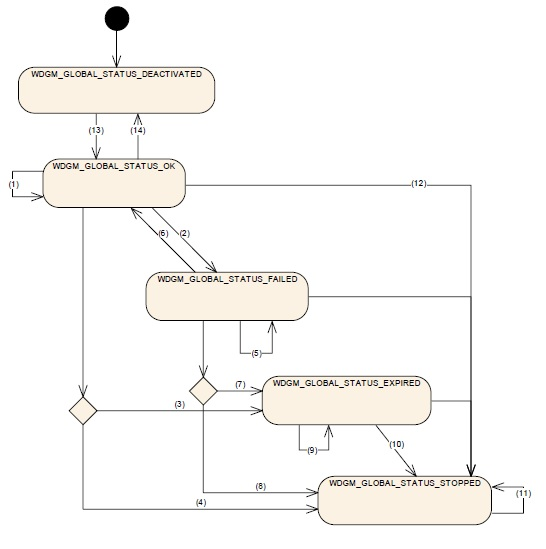
\includegraphics{pictures/globalstatuses}
  \label{APP:FIG:GLOBALSTATUS}
  \caption{The possible global statuses represented as a graph}
\end{figure}

\section{Local Status}
A local status is a status of one supervised entity and could be set according
to the current local status and the results of the supervision functions. There
are four different local statuses. Init setmode mainfunction

\begin{itemize}
  \item WDGM\_LOCAL\_STATUS\_DEACTIVATED\\
    If a supervised entity is set to deactivated, it will not be checked by the
    supervision functions.
  \item WDGM\_LOCAL\_STATUS\_OK\\
    The supervised entity is in a correct state.
  \item WDGM\_LOCAL\_STATUS\_FAILED\\
    Alive supervision for the supervised function has failed.
  \item WDGM\_LOCAL\_STATUS\_EXPIRED\\
    A fault has been observed within the supervised function. The main function
    will save the identification of the first supervised entity which reach this
    state.
\end{itemize}
Figure \ref{APP:FIG:LOCALSTATUSES} describes the state machine for the local
status of a supervised entity.

\begin{figure}[!ht]
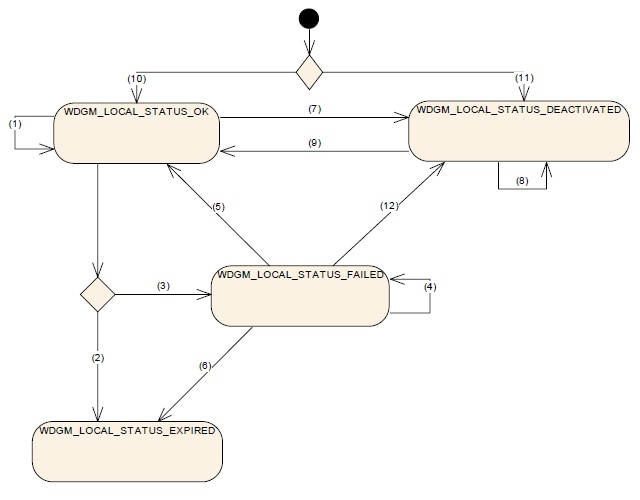
\includegraphics{pictures/localstatuses}
\label{APP:FIG:LOCALSTATUSES}
\caption{The possible local statuses represented as a graph}
\end{figure}

\section{API functions}
\label{APP:API_CALLS}
\subsection{WdgM\_Init}
Initializes the watchdog manager by setting, among other things, the local
status of all supervised entities to either WDGM\_LOCAL\_STATUS\_OK or
WDGM\_LOCAL\_STATUS\_DEACTIVATED. It also changes the global status to
WDGM\_GLOBAL\_STATUS\_OK.
\subsection{WdgM\_DeInit}
De initializes the watchdog manger.
\subsection{WdgM\_GetVersionInfo}
Returns the version info of the watchdog manager module.\footnote{The function shall not change the
internal state of the watchdog manager and should be side effect free.}
\subsection{WdgM\_SetMode}
Sets a new mode for the watchdog manager.
\subsection{WdgM\_GetMode}
Returns the current mode for the watchdog manager\footnotemark[\thefootnote].
\subsection{WdgM\_CheckpointReached}
\label{SEC:CHECKPOINTREACHED}
Performs deadline and logical supervision for a given supervised entity.
\subsection{WdgM\_GetLocalStatus}
Returns the local status of a supervised entity\footnotemark[\thefootnote].
\subsection{WdgM\_GetGlobalStatus}
Return the global status of the watchdog manager\footnotemark[\thefootnote].
\subsection{WdgM\_PerformReset}
Shall set the trigger condition for all configured watchdogs to zero and
thereby causing the hardware watchdogs to cause an external hardware reset.
\subsection{WdgM\_GetFirstExpiredSEID.}
Returns the supervised entity that first reached the state
\emph{WDGM\_LOCAL\_STATUS\_EXPIRED}\footnotemark[\thefootnote].
\subsection{WdgM\_MainFunction}
\label{SEC:MAINFUNCTION}
The main function is periodically called, it first updates the local statuses by
running alive supervision for the supervised entities and then sets the global
status depending on the current state of the watchdog manager; this includes the
new values of the local statuses.

%%%%%%%%%%%%%%%%%%%%%%%%%%%%%%%%%%%%%%%%%%%%%%%%%%%%%%%%%%%%%%%%%%%%%%%%%%%%%%%%

\setlength{\parindent}{0pt}
%% \begin{comment}
\chapter{Bugs in C-code}
\section{Failed reference supervision cycles is changed to early}
When applying the requirements [WDGM203], [WDGM204], [WDGM300], [WDGM205], the counter for failed reference cycles has already been
changed. The old value for the counter is needed.

\subsection{Severity}
Significant

\subsection{Steps to reproduce}
\begin{lstlisting}
WdgM_Init(Configuration)
WdgM_SetMode(0, 1)
WdgM_MainFunction()
WdgM_MainFunction()
WdgM_MainFunction()
WdgM_MainFunction()
WdgM_MainFunction()
\end{lstlisting}
\paragraph{Expected results:}
The global status should be \lstinline!WDGM_GLOBAL_STATUS_EXPIRED!.
\paragraph{Actual results:}
The global status is set to \lstinline!WDGM_GLOBAL_STATUS_FAILED!.

\subsection{Further comments}
There is possibly some additional unwanted behavior because of this,
that one should be aware of.

Because of the alive supervision results does not change appropriately
with the local status of the supervised entity, there is a possibility
where you don't reach the requirements [WDGM300] or [WDGM205], because
the alive supervision result is still \lstinline!WDGM_INCORRECT! when it should be
\lstinline!WDGM_CORRECT!, and the local status is \lstinline!WDGM_LOCAL_STATUS_FAILED!.

When testing the additional configuration, which only contains alive
supervision we found that the sequence:
\begin{lstlisting}
WdgM_Init(Configuration)
WdgM_SetMode(0, 1)
WdgM_MainFunction()
WdgM_MainFunction()
WdgM_CheckpointReached(0, 4)
WdgM_CheckpointReached(0, 4)
WdgM_MainFunction()
WdgM_MainFunction()
\end{lstlisting}
gives a state where the local status for a supervised entity (with ID
0) was\\\lstinline!WDGM_LOCAL_STATUS_FAILED! which is correct, but the alive
supervision result for that checkpoint was \lstinline!WDGM_INCORRECT!, where it
should have been\\\lstinline!WDGM_CORRECT!.

We don't know if this is a reproducable behaviour after this bug is
fixed, but it should be good to do an additional check.

\section{CheckpointReached overwrites results from logical
  supervision}
If there are N graphs for internal logical supervision for a
supervised entity, then you derive N results from internal logical
supervision. The same goes for external logical supervision; if you
got M graphs for external logical supervision for a supervised entity,
you got M results.

Then for that supervised entity, you got N+M results from logical
supervision. This is specified in 7.2.3.2.
CheckpointReached overwrites the results from earlier executions.

\subsection{Severity}
Medium

\subsection{Steps to reproduce}
\begin{lstlisting}
WdgM_Init(Configuration)
WdgM_SetMode(1, 1)
WdgM_CheckpointReached(3, 23)
WdgM_CheckpointReached(3, 19)
WdgM_CheckpointReached(3, 23)
WdgM_CheckpointReached(3, 20)
\end{lstlisting}
\paragraph{Expected result:}
The results from logical supervision for the supervised entity should
be set to \lstinline!WDGM_INCORRECT!, due to the external graph (3,23) fails.
\paragraph{Actual result:}
The results from logical supervision is set to \lstinline!WDGM_CORRECT!.

\section{Possible wrong behaviour after two WdgM\_CheckpointReached calls}
In logical supervision, if the activity flag for a graph is false (the
logical graph has not been started), and a checkpoint that is not
initial is reached through \lstinline!WdgM_CheckpointReached!, the logical
supervision result for that supervised entity is set to
\lstinline!WDGM_INCORRECT!, and the local status is set to
\lstinline!WDGM_LOCAL_STATUS_EXPIRED!.

However, if a correct checkpoint is reached after the faulty/incorrect
checkpoint, \lstinline!WdgM_CheckpointReached! will set the logical supervision
result and the local status to \lstinline!WDGM_CORRECT! and \lstinline!WDGM_LOCAL_STATUS_OK!,
respectively.  The chapter 7.2.3 in AUTOSAR, WatchdogManager, states
``Logical supervision checks if the code of supervised entities is
executed in the correct sequence.''.  There is no requirements for this
specific case, and AUTOSAR is unclear of what should happend. Still it
would be nice to not overwrite the results of logical supervision.

\subsection{Severity}
Proposed change

\subsection{Steps to reproduce}
\begin{lstlisting}
WdgM_Init(Configuration)
WdgM_SetMode(0, 1)
WdgM_CheckpointReached(2, 13)
WdgM_CheckpointReached(2, 12)
\end{lstlisting}
\paragraph{Expected results:}
The local status may have stayed in \lstinline!WDGM_LOCAL_STATUS_EXPIRED!.
\paragraph{Actual results:}
The local status is \lstinline!WDGM_LOCAL_STATUS_OK!.

\subsection{Other remarks}
The effect of the bug ``CheckpointReached overwrites results from
logical supervision'' is that the results from different graphs are
overwritten, while the effect of this bug is that the result from the
same graph are overwritten.


\section{DeInit changes the global status even if it shouldn't}
The function \lstinline!WdgM_DeInit! sets the global status to
\lstinline!WDGM_GLOBAL_STATUS_DEACTIVATED! even if the global status was not in
\lstinline!WDGM_GLOBAL_STATUS_OK!. The requirement that is violated is [WDGM286],
and figure 4 (the global status state machine). This could have
dangerous consequences.

\subsection{Severity}
Significant

\subsection{Steps to reproduce}
\begin{lstlisting}
WdgM_Init(Configuration)
WdgM_CheckpointReached(0, 1)
WdgM_MainFunction()
WdgM_DeInit()
\end{lstlisting}
\paragraph{Expected Results:}
Global status should stay in \lstinline!WDGM_GLOBAL_STATUS_EXPIRED!.
\paragraph{Actual Results:}
Global status is set to \lstinline!WDGM_GLOBAL_STATUS_DEACTIVATED!.

\section{Supervised entities initialized to wrong value\\(WDGM\_INCORRECT)}
\lstinline!WdgM_Init! initializes the results of supervision functions for all
supervised entities to \lstinline!WDGM_INCORRECT!. This violates page 27 of
AUTOSAR, claiming ``At Watchdog Manager initialization, all the Results
are set to correct''.

\subsection{Severity}
Significant

\subsection{Other remarks}
This is a problem with the generated files, so a function call is not
needed to reproduce this bug.

\section{SetMode does not retain the state for supervised entitites}
The AUTOSAR requirement [WDGM182] claims that ``each Supervised Entity
that is activated in the new mode, the function \lstinline!WdgM_SetMode! shall
retain the current state of the Supervised Entity.''

\subsection{Severity}
Significant

\subsection{Steps to reproduce}
\begin{lstlisting}
WdgM_Init(Configuration)
WdgM_SetMode(0, 1)
WdgM_MainFunction()
WdgM_MainFunction()
WdgM_SetMode(0, 1)
\end{lstlisting}
\paragraph{Expected Results:}
At least one supervised entity should be in \lstinline!WDGM_LOCAL_STATUS_FAILED!
and have one supervision result set to \lstinline!WDGM_INCORRECT!.
\paragraph{Actual Results:}
All supervised entities was reseted.

\section{Internal logical supervision should fail when a checkpoint is not an initial one}
In internal logical supervision, if a checkpoint belonging to a
internal graph is not an initial checkpoint, and the activity flag for
that graph is false, then the function \lstinline!WdgM_CheckpointReached! should
set the logical supervision for that supervised entity to
\lstinline!WDGM_INCORRECT\lstinline!, according to the requirement [WDGM274].

\subsection{Severity}
Significant

\subsection{Steps to reproduce}
\begin{lstlisting}
WdgM_Init(Configuration)
WdgM_SetMode(0, 1)
WdgM_CheckpointReached(2, 13)
\end{lstlisting}
\paragraph{Expected Results:}
Logical supervision for supervised entity with ID 2 is supposed to be
\lstinline!WDGM_INCORRECT!.
\paragraph{Actual Results:}
Logical supervision for supervised entity with ID 2 is after execution
set to \lstinline!WDGM_CORRECT!.

\section{External logical supervision should fail when a checkpoint is
  not an initial one}
In external logical supervision, if a checkpoint belonging to an
external graph is not an initial checkpoint, and the activity flag for
that graph is false, then the function \lstinline!WdgM_CheckpointReached! should
set the logical supervision for that supervised entity to
\lstinline!WDGM_INCORRECT!, according to the requirement [WDGM252].

\subsection{Severity}
Significant

\subsection{Steps to reproduce}
\begin{lstlisting}
WdgM_Init(Configuration)
WdgM_SetMode(0, 1)
WdgM_CheckpointReached(1, 7)
\end{lstlisting}
\paragraph{Expected Results:}
Logical supervision for supervised entity with ID 1 is supposed to be
\lstinline!WDGM_INCORRECT!.
\paragraph{Actual Results:}
Logical supervision for supervised entity with ID 1 is after execution
set to \lstinline!WDGM_CORRECT!.

\section{Incorrect increment of the expired cycle counter}
The counter for ``expired cycle counter'' is incremented when the
\lstinline!WdgM_MainFunction! changes the global state from \lstinline!WDGM_GLOBAL_STATUS_OK!
or\\\lstinline!WDGM_GLOBAL_STATUS_FAILED! to \lstinline!WDGM_GLOBAL_STATUS_EXPIRED! or
\lstinline!WDGM_GLOBAL_STATUS_STOPPED!, violating [WDGM215],[WDGM216],[WDGM077],
and [WDGM117]. This has the consequences that violates [WDGM219], and
[WDGM220].  The expired cycle counter should not be incremented in the
first round.

\subsection{Severity}
Significant

\subsection{Steps to reproduce}
\begin{lstlisting}
WdgM_Init(Configuration)
WdgM_SetMode(0, 1)
WdgM_CheckpointReached(0, 1)
WdgM_MainFunction()
WdgM_MainFunction()
WdgM_MainFunction()
\end{lstlisting}
\paragraph{Expected results:}
The global status should be \lstinline!WDGM_GLOBAL_STATUS_EXPIRED! for one more round.
\paragraph{Actual results:}
The global status is \lstinline!WDGM_GLOBAL_STATUS_STOPPED!.

\section{WdgM\_Init does not reset activity flags for graphs}
\lstinline!WdgM_Init! should reset the activity flag for each graph (both
external and internal) in logical supervision according to [WDGM296].

\subsection{Severity}
Medium

\subsection{Steps to reproduce}
\begin{lstlisting}
WdgM_Init(Configuration)
WdgM_SetMode(0, 1)
WdgM_CheckpointReached(2, 12)
WdgM_DeInit()
WdgM_Init(Configuration)
WdgM_SetMode(0, 1)
WdgM_CheckpointReached(2, 12)
\end{lstlisting}
\paragraph{Expected results:}
The logical supervision results for supervised entity with ID 2 should
be \lstinline!WDGM_CORRECT!.
\paragraph{Actual results:}
The results for logical supervision is set to \lstinline!WDGM_INCORRECT!.

\section{WdgM.h has wrong case of an include file}
In WdgM.h the file WdgM\_Pbcfg.h is (incorrectly) included as
``WdgM\_PbCfg.h'', notice the uppercase C in the filename.

\subsection{Severity}
Uncritical

\section{WdgMSupervisionCycle configuration parameter in wrong
  container}
The configuration parameter WdgMSupervisionCycle should be in each
WdgMMode-container, and not in WdgMGeneral according to requirement
[WDGM330\_Conf]. This makes it impossible for \lstinline!WdgM_Init! to check the
requirement [WDGM010]. I think there should be a check against this
in the generator (picea\_wdgm\_scg.exe).

\subsection{Severity}
Medium

\subsection{Integration impact}
The WdgMSupervisionCycle parameter is added in the WdgMMode container
(as optional) and will override the parameter located in
WdgMGeneral. An error will be thrown if the WdgMSupervisionCycle
parameter is missing in both the WdgMMode and WdgMGeneral.


\section{WdgM initiates the global status to\\
  WDGM\_GLOBAL\_STATUS\_OK}
WdgM initiates the global status to \lstinline!WDGM_GLOBAL_STATUS_OK!.
This violates figure 4 in AUTOSAR (page 34) and possibly [WDGM285].

\subsection{Severity}
Medium

\subsection{Steps to reproduce}
\begin{lstlisting}
WdgM_DeInit()
\end{lstlisting}
\paragraph{Expected result:}
Global status should be in \lstinline!WDGM_GLOBAL_STATUS_DEACTIVATED!.
\paragraph{Actual result:}
Global status is set to \lstinline!WDGM_GLOBAL_STATUS_OK!.

%% \end{comment}

%%%%%%%%%%%%%%%%%%%%%%%%%%%%%%%%%%%%%%%%%%%%%%%%%%%%%%%%%%%%%%%%%%%%%%%%%%%%%%%%

\chapter{Ambiguities in AUTOSAR}
% \subsection*{Bad transition}
% Stated by [WDGM285], ``if \lstinline!WdgM_Init! was successfully called, change
% global supervision status to \lstinline!WDGM_GLOBAL_STATUS_OK!''.

% [WDGM139] claims that ``if a call to \lstinline!WdgIf_SetMode! fails,
% the function shall assume a global supervision failure and set the
% global supervision status to \lstinline!WDGM_GLOBAL_STATUS_STOPPED!'',
% with a reference to the transition between
% \lstinline!WDGM_GLOBAL_STATUS_OK! and stopped.

% What if it were not successfully called?

% If \lstinline!WdgIf_SetMode! is not successfully called, how can
% \lstinline!WdgM_Init! be successfully, and get the global status
% \lstinline!WDGM_GLOBAL_STATUS_OK!?


\section{Incorrect reference}
\subsection{Requirement description}
\paragraph{[WDGM273]} If the function
\lstinline!WdgM_CheckpointReached! determines that the result of the
Logical Supervision for the given Checkpoint is true, and the
Checkpoint is the \colorbox{yellow}{initial} one
(\colorbox{yellow}{WdgMInternalCheckpointInitialRef}), then shall set
the Activity Flag of the Graph corresponding to the Checkpoint to
\colorbox{yellow}{true}. (BSW09221, BSW09222)

\paragraph{[WDGM329]} If the function
\lstinline!WdgM_CheckpointReached! determines that the result of the
Logical Supervision for the given Checkpoint is true, and the
Checkpoint is the \colorbox{yellow}{initial} one
(\colorbox{yellow}{WdgMInternalCheckpointFinalRef}), then shall set
the Activity Flag of the Graph corresponding to the Checkpoint to
\colorbox{yellow}{true}. ()

\subsection{Problem description}
Both requirements \textbf{[WDGM273]} and \textbf{[WDGM329]} refers to
a ``initial'' checkpoint, but one of the requirements (preferably
\textbf{[WDGM329]}) should instead refer to a ``final'' checkpoint. It
should in that case also set the activity flag of the corresponding
graph to false.

\section{Optional or mandatory}
\subsection{Requirement description}
\paragraph{[WDGM344]} If development error detection for the Watchdog
Manager module is enabled, then the function \lstinline!WdgM_GetGlobalStatus!
shall check whether the parameter Status is a NULL pointer
(NULL\_PTR). If Status is a NULL pointer, then the function shall raise
the development error \lstinline!WDGM_E_INV_POINTER! (i.e. invalid pointer) and
return.  ()

There are \colorbox{yellow}{optional} checks that are executed if and
only if WdgMDevErrorDetect is enabled.
\paragraph{[WDGM258]} If the configuration parameter WdgMDevErrorDetect
[WDGM301\_Conf] is enabled, the routine shall check if NULL pointers
are passed for OUT parameters. In case of an error the service shall
not be executed, the error shall be reported to the Development Error
Tracer with the error code \lstinline!WDGM_E_INV_POINTER! and the routine shall
return the value \lstinline!E_NOT_OK!.  (BSW00323)

\subsection{Problem description}
The requirements \textbf{[WDGM344]} and \textbf{[WDGM258]} describes
the same actions, with one difference: one is optional, the other mandatory.

\section{Logical supervision results}
\subsection{Problem description}
AUTOSAR does not specify if it is possible to overwrite logical supervision
results from the same supervised entity.

I.e.
\begin{lstlisting}
  WdgM_CheckpointReached(SEx, Bad_CP)  -> incorrect result for SEx
  WdgM_CheckpointReached(SEx, Good_CP) -> Correct result for SEx
\end{lstlisting}

\section{Incorrect spelling}
\subsection{Requirement description}
\begin{tabular}{| l | l |} \hline
SWS Item & \textbf{[WDGM344\_CONF]}\\\hline
Name     & \colorbox{yellow}{WdgMInternallCheckpointFinalRef}\\\hline
Description & This is the reference to the final Checkpoint(s) for
this Supervised Entity.\\\hline
\end{tabular}

\paragraph{[WDGM315]} If the current global status is
\lstinline!WDGM_GLOBAL_STATUS_OK! or
\lstinline!WDGM_GLOBAL_STATUS_FAILED! then for each Supervised Entity
that is deactivated in the new mode (passed to function
\lstinline!WdgM_SetMode! as parameter), the function
\lstinline!WdgM_SetMode! shall change the state of the Supervised
Entity to\\\lstinline!WDGM_LOCAL_STATUS_DEACTIVATED!; It shall set its
Results of \colorbox{yellow}{Active}, Deadline and Logical Supervision
to correct; It shall also clear its failed reference cycle counter to
0.

\subsection{Problem description}
Requirement \textbf{[WDGM344\_CONF]} has miss spelled its name
\textit{WdgMInternallCheckpointFinalRef}. This differs from references
in other requirements, for example in \textbf{[WDGM329]}.

\section{Retain state}
\subsection{Requirement description}
\paragraph{[WDGM182]} If the current global status is
\lstinline!WDGM_GLOBAL_STATUS_OK! or
\lstinline!WDGM_GLOBAL_STATUS_FAILED! then for each Supervised Entity
that is activated in the new mode (passed to function
\lstinline!WdgM_SetMode! as parameter), the function
\lstinline!WdgM_SetMode! shall \colorbox{yellow}{retain the current
state of the Supervised Entity}.  Switching to the mode where a
Supervised Entity is deactivated clears also errors that had resulted
with the \lstinline!WDGM_GLOBAL_STATUS_FAILED!  status. ()

\subsection{Problem description}
The problem is that it is unclear what the supervised entity state
should contain. We know that the status, the results of alive,
deadline and logical supervision and some counters should be part of
this state. Should the supervision functions be part of the state?

This could be problematic because then there is a need to map out
which supervision function should be retained (exists in the new mode
as well as the old mode), which should be discarded (does not exist in
the new mode) and which should be created (exists in the new mode but
not the old).

If it is not part of the state, then all supervisions functions should
be discarded and the new supervision functions should be added.  This
could also be problematic because, what if there exist a supervision
function which has the status \lstinline!WDGM_INCORRECT!  and the only
thing that keeps the supervised entity from setting the status\\
\lstinline!WDGM_LOCAL_STATUS_EXPIRED! is a call to
\lstinline!WdgM_MainFunction!. Then a call to \lstinline!WdgM_SetMode!
with the same mode could reset all supervision functions and the
expired state would not happen.

Another question arises; should internal logical supervision functions
count? They are mode independent, but if the supervised entity is
deactivated, the internal logical supervision should not be able to do
anything.

%% \subsection*{Definition of time in deadline supervision}
